\documentclass[a4paper, 10pt]{article}
\usepackage[T1]{fontenc}
\usepackage{tgpagella}
\usepackage[english]{babel}
\usepackage{amsmath,amsfonts,amssymb,amsthm}
%\usepackage{mathtools}
\usepackage{graphicx}
\usepackage{xcolor}
\usepackage{setspace}
\usepackage{amssymb,amsmath,amsfonts,booktabs,eurosym,geometry,ulem,graphicx,caption,color,setspace,sectsty,comment,footmisc,caption,natbib,pdflscape,subfigure,array,bbm}

\usepackage[colorlinks=true,linkcolor=red,linkcolor={black},citecolor={black}]{hyperref}
\normalem
\onehalfspacing
\newcommand\tinghuan[1]{\textcolor{blue}{{Tinghuan: }{#1}}}
\newcommand\oliver[1]{\textcolor{olive}{{Oliver: }{#1}}}
\newcommand\wenjie[1]{\textcolor{purple}{{Wenjie: }{#1}}}

\newcommand{\red}[1]{{\color{red} #1}}
\newcommand{\blue}[1]{{\color{blue} #1}}

\newcolumntype{L}[1]{>{\raggedright\let\newline\\arraybackslash\hspace{0pt}}m{#1}}
\newcolumntype{C}[1]{>{\centering\let\newline\\arraybackslash\hspace{0pt}}m{#1}}
\newcolumntype{R}[1]{>{\raggedleft\let\newline\\arraybackslash\hspace{0pt}}m{#1}}
\geometry{left=1.0in,right=1.0in,top=1.0in,bottom=1.0in}





\title{%
\begin{center}
    
\includegraphics[scale=0.15]{figures/UZH2.png}
\end{center}
\vspace{4em}
%     \textsc{The Effect of Conditional Cash Transfers on School Attendance - A Meta Analysis Approach}
     \textsc{Conditional Cash Transfers and School Attendance:\\A Meta-Analytical Approach}
}
\author{Tinghuan Liu\thanks{Student ID: 20-742-391} \and Oliver Pedrini \thanks{Student ID: 15-933-732}\and Wenjie Tu\thanks{Student ID: 20-740-916} }
\date{Fall Semester 2021}\setlength{\parindent}{0pt}
%\setlength{\parskip}{1em}
% \doublespacing
\setlength{\parskip}{1em}
%\setcounter{page}{0}

% Please use the command here to make your comment directly on the project
% Example:
% \wenjie{This is a comment.} 



\begin{document}

\clearpage
\maketitle
\thispagestyle{empty}

\begin{abstract}
\noindent We reexamined the effect that conditional cash transfers have on school attendance of children in the age range 11-16 years old through a meta-analytical approach using a selection of 10 studies. We found that on average conditional cash transfers result in an increase of school attendance of 4 percentage points. We also found no strong evidence of publication bias. However, we failed to address the large degree of between-study heterogeneity of the selected studies.

\vspace{4mm}

\noindent\textbf{Keywords:} Conditional Cash Transfers; School Attendance; Meta-Analysis; CCT


\end{abstract}

\newpage

%\setcounter{page}{1}

\doublespacing

% -------------------------------------------------------------------------------------
\section{Introduction} \label{sec:introduction}

\begin{comment}
Education plays an important role in the development process. At an individual level, education is a fundamental way of accumulating human capital and an essential channel to avoid poverty transmission across generations (\cite{angrist1991does}, \cite{duflo2004medium} and \cite{tilak2002education}). At a country level, education is irreducible for technological progress and will ultimately contribute to growth convergence (\cite{barro2001human}, \cite{krueger2001education} and among others). 

Even though education is crucial for development, relatively low school attendance is a problem for developing countries. Compared with developed countries, enrollment ratios in secondary education are usually much lower in developing countries and could be even lower for children from low income families.\footnote{https://ourworldindata.org/global-education}

Among all reasons, liquidity constraints and perceived low returns on education by parents are considered as two straightforward reasons for relatively low school attendance rate in developing countries (\cite{baland2000child} and \cite{doi:10.1146/annurev.economics.050708.143323}). Specifically, when households face with liquidity constraints, it is more likely that they allocate less money to children’s education expense. On the other hand, as parents make the decision whether to send child to school, they are tradeoffing the return of labor participation at the present with children’s future education return. If the return on education is perceived lower by parents, they might also forge education to their children.

Considering above two barriers for school attendance, many governments and non-governmental organizations have been rolling out conditional cash transfer (CCT) programs that transfer money to household conditional on making a series of human capital investments in their young children in the past 40 years.\footnote{There are two types of cash transfers - unconditional cash transfers and conditional cash transfers. Unconditional cash transfers offer the targeted people cash without requiring any behavioral changes. Conditional cash transfers instead require beneficiaries to engage in some productive behaviour such as investing in their education or health.} Straightforwardly, transferring cash specified for young children’ education could hopefully mitigate the budget constraint of household, and increase the return of education by reducing its cost. Also due to the mechanical feature of conditional transfer, it could also avoid the time-inconsistence problem from the household. 


It is also noticeable that conditional cash transfer is the most popular social programs in the developing world. Over 63 countries have at least one CCT program and those programs have covered millions of families worldwide ( World  \cite{bank2018state}). The popularity of CCT program proliferates many empirical studies investigating the casual effect of conditional cash transfer on school attendance in developing countries. XXX find positive effect with magnitude ranging from, while XXX find negative effect. 

Here we revisit this question by a meta-analysis approach. The marginal contribution of our paper could be seen from three respects. Firstly, as there have been enough empirical studies directly examining their relationship, this materializes the opportunity to systematically summarize those studies. By meta-analysis, we could  efficiently aggregate all the existing studies to get a more accurate estimate. 

Secondly, though most studies find positive effect of CCT, the magnitude of estimation vary a lot. \cite{Barrera-Osorio2017} argues that the heterogeneity of different implement of programs play a big role of these difference. It is possible that the positive effect of CCT on school attendance depend crucially on other context variables other than CCT itself. For example, most studies find positive effect when the targeting place is located in South America, it might be the targeting place cause the positive effect other than CCT itself. In this paper, we will explicitly control those heterogeneity through random effect model.

In addition to heterogeneity of different studies, publication bias might also cast doubt on the positive effect of CCT. \cite{brodeur2018methods} documents a serious publication bias among empirical literature. Applying this consideration into our case, if the seemingly consistent positive effect of CCT comes from bias publication, it would be likely that the underlying true effect is not positive if we could account other unpublished papers. In this paper, we will explicitly account the bias coming from publication through meta regression method. 


In this paper, we find significantly positive impact of CCT programs on school attendance from fixed effect and random effect model. However, when the publication bias and between-study heterogeneity are accounted, the statistically significant result vanished and even became negative in most regression specifications. These results may indicate either the disturbance from heterogeneity of different studies or the P-hacking behavior from publication incentive.   

This rest paper is organized as follows. Section 2 overviews the prior evidence on the relationship between conditional cash transfers and school attendance. Section 3 explains the detailed procedure following which we collect our data. Section 4 is the main part of this paper, which presents the results from meta analysis and meta-regression. Finally, Section 5 concludes.
\end{comment}

% Oliver's edit
Education plays an important role in the development process. At an individual level, education is an important way to accumulate human capital and an essential channel to avoid poverty transmission across generations (\cite{angrist1991does}, \cite{duflo2004medium} and \cite{tilak2002education}). At a country level, education is strongly tied to technological progress, which is essential to economic growth (\cite{barro2001human} and \cite{krueger2001education}, among others).

Even though education is crucial for development, relatively low school attendance is a problem for developing countries. Compared with developed countries, enrollment ratios in secondary education are usually much lower in developing countries and could be even lower for children from low income families.\footnote{https://ourworldindata.org/global-education} %\textbf{Data on school attendance, not enrolment} 

Among all reasons, liquidity constraints and perceived low returns on education by the parents are considered reasons for the relatively low school attendance rates in developing countries (\cite{baland2000child} and \cite{doi:10.1146/annurev.economics.050708.143323}). Specifically, when households face liquidity constraints, it is more likely that they allocate less money to the children’s educational expenses, as for the parents the trade-off of investing money and time in education for their children in exchange of its future returns is less appealing.

Several governments and non-governmental organizations have been rolling out conditional cash transfer (CCT)\footnote{There are two types of cash transfers: unconditional cash transfers and conditional cash transfers. Unconditional cash transfers offer the targeted people cash without requiring any action by the recipient. Conditional cash transfers instead require beneficiaries to engage in some desirable behaviours such as enrolling to school and regularly visiting the doctor.} programs that transfer money to households on the condition of making some kind investment in their children's human capital. Returning to the content of the previous paragraph, transferring cash aimed to young children’s education could mitigate the budget constraints of the households.

It is also worth observing that CCTs are among the most popular social programs in the developing world. Over 63 countries have at least one CCT program and those programs have covered millions of families worldwide (World  \cite{bank2018state}). The popularity of CCT programs has lead to a vast literature. Here we revisit the impact that CCT programs have on school attendance with a meta-analytical approach. We want to try to aggregate existing literature on the topic and obtain a clear reading of the causal relationship.

Other than the heterogeneity of the different studies, publication bias might also cast doubt on the positive effect of CCTs. \cite{brodeur2018methods} document a serious problem of publication bias among empirical literature. Therefore, we also investigated the presence of publication bias in our sample of studies. 

Our initial analysis found a significantly positive relation between CCT programs and school attendance when using fixed-effects and random-effects models. We did not find strong evidence of publication bias in our investigation, therefore the initial results remain robust under the publication bias hypothesis. Finally, we tried to address the high heterogeneity between the selected studies, but failed to find any factor driving it.

The rest of the article is structured as follows: section \ref{sec:evidence} gives an overview of prior literature on the relationship between CCTs and school attendance. Section \ref{sec:data} reports the protocol we applied when searching the literature, selecting the relevant studies and extracting the data from them. In section \ref{sec:results} we conduct our meta-analytical research. Finally, Section \ref{sec:conclusion} concludes.


% -------------------------------------------------------------------------------------
\section{Literature Review} \label{sec:evidence}

\begin{comment}
% There have been several prior empirical studies which test for the relationship between conditional cash transfers and school attendance. To summarize their conclusions, most studies find conditional cash transfers have a positive impact on school attendance. 

There is an increasing awareness that investment in human capital at an early age can have significant impacts on social mobility at an individual level and on economic growth at a national level. This notion is the basis for the popularity of conditional cash transfer programs to help boost children’s education outcomes. There have been some empirical studies investigating the relationship between CCTs and school attendance. To summarize their findings, most studies indicate a positive and significant impact of CCTs on school attendance. Several studies, however, show no evidence that CCTs programs can improve school attendance.



\cite{akresh2013cash} provide empirical evidence for the positive relationship between CCTs and school attendance. It is argued that CCTs are significantly more effective than UCTs in improving the enrollment of ``marginal children'' who are initially less likely to go to school such as girls, younger children, and lower-ability children. \cite{Barrera-Osorio2017} show that CCT treatment does increase enrollment rates at both the secondary and tertiary levels. It is also argued that changing the timing of the payments does not change attendance rates relative to the basic CCT treatment. \cite{Edo2017} estimate that the CCT program accounts for a 3.9 percentage point increase in the probability of attending secondary school among eligible children aged from 15 to 17. \cite{Filmer2011} find that a modest cash transfer, equivalent to approximately 2\% of the consumption of the median recipient household, had a substantial impact on school attendance, approximately 25 percentage points.  \cite{levy2010} identify positive and statistically significant impacts on school attendance. However, they find no evidence that the CCT program has an impact on long-term outcomes such as marks and grade progression. \cite{Perova2012} reveal a considerable increase (25 percentage points) in the likelihood of beneficiary children attending school with the CCT intervention.

However, several studies suggest that CCTs programs have negligible impacts on school attendance. \cite{Armand2018} examine the short- and medium-run impacts of CCTs on school enrollment and finds that the CCT program has strong impacts on school enrollment among children of secondary school age, but not on school attendance. \cite{Borraz2009} analyze the impact of CCTs on school enrollment and no significant impact is detected on school attendance. \cite{Corrales2020} suggest that the CCT program does not always manage to bring into line the school attendance of children from families involved in the program with that of similar families not in the program.  \cite{Ferre2014} show that the CCT intervention was not able to improve school attendance. 

Overall, the evidence on the impact of CCTs on school attendance is mixed. Most studies suggest a positive relationship between CCTs and school attendance. However, some argue that one cannot attribute these results to CCT programs. An underlying heterogeneity such as family and innate ability among beneficiaries may play a role. Hence, several studies also reveal no impact on school attendance. Our research is built on these empirical findings. By using a meta-analysis approach, we try to aggregate these findings and summarize the overall effect of CCTs on school attendance.
\end{comment}

% https://academia.stackexchange.com/questions/121769/is-a-citation-typically-considered-plural-or-singular-in-academia
% To keep consistent, a citation refers to authors not the paper although it could refer to the paper 

% Oliver's edit
There is an increasing awareness that investment in human capital at an early age can have significant impacts on social mobility at an individual level and on economic growth at a national level. This notion is the basis for the popularity of CCT programs to help boosting children’s educational outcomes. There have been some empirical studies investigating the relationship between CCTs and school attendance. To summarize their findings, most studies indicate a positive and significant impact of CCTs on school attendance. A part of the studies, however, find no evidence that CCTs programs can improve school attendance.

\cite{akresh2013cash} provide empirical evidence for the positive relationship between CCTs and school attendance. It is argued that CCTs are significantly more effective than UCTs in improving the attendance of "marginal children'' who are initially less likely to go to school such as girls, younger children, and lower-ability children. \cite{Barrera-Osorio2017} find that the CCT treatment does increase attendance. \cite{Edo2017} estimate that the CCT program accounts for a 3.9 percentage points increase in the probability of attending secondary school among eligible children aged from 15 to 17. \cite{Filmer2011} find that a modest cash transfer, equivalent to approximately 2\% of the consumption of the median recipient household, had a substantial impact on school attendance, approximately a 23 percentage points increase. \cite{levy2010} identify some positive and statistically significant impacts on school attendance. However, they find no evidence that the CCT program had an impact on long-term outcomes such as marks and grade progression. \cite{Perova2012} find a significant increase in school attendance during the second year of the CCT program. \cite{Corrales2020} suggest that the considered CCT program affects school attendance of children 12 to 17 years old, while it does not for children 6-11 years old.

Some other studies suggest that CCT programs have negligible impacts on school attendance. \cite{Armand2018} examine the short and medium-run impacts of CCTs on school enrollment and find that the considered CCT program had strong impacts on school enrollment among children of secondary school age, but not on school attendance. \cite{Borraz2009} analyze the impact of CCTs on school enrollment and no significant impact is detected on school attendance. \cite{Ferre2014} suggest that the CCT intervention was not able to improve school attendance.

Overall, the evidence on the impact of CCTs on school attendance is mixed. Most studies suggest a positive relationship between CCTs and school attendance. However, some argue that one cannot attribute these results to CCT programs. An underlying heterogeneity such as family background and innate ability among beneficiaries may play a role. Hence, several studies also reveal no impact on school attendance. Our research is built on these empirical findings. Using a meta-analytical approach we try to aggregate these findings and summarize the overall effect of CCTs on school attendance.

% -------------------------------------------------------------------------------------
\section{Data} \label{sec:data}

In this section, we describe how we searched through the literature, selected the studies that are useful for our research and how we extracted the needed data from them.

\subsection{Search for Studies}


We conducted a thorough literature search for empirical studies investigating the effect of CCTs on school attendance. We used Google Scholar as our primary search engine with the keywords ``\textit{Conditional Cash Transfers AND School Attendance}'', ``\textit{Conditional Cash Transfers AND Education}'', ``\textit{Conditional Cash Transfer AND Schooling}'' and ``\textit{Conditional Cash Transfer AND Attendance}''. We also searched through the Web of Science database using the same keywords. Lastly, we also followed citations and references of the studies we collected to find other unpublished or yet undiscovered studies.

% -------------------------------------------------------------------------------------
\subsection{Criteria for Eligibility} 

To decide whether or not a study was suitable to be included in our dataset, we applied the following selection criteria:
\begin{itemize}
    \item The study explores the impact that CCTs have on school attendance.
    \item The study has to be written in English. We opted for English only studies, because we wanted everyone in our research team to be able to access them, even if we could have considered other languages, such as Chinese, Italian and possibly Spanish.
    \item The effect should include at least part of the age range that goes from 11 to 16 years old as the affected category. We focus our study to this specific age range to avoid heterogeneity caused by different effects for different age ranges.
    \item The study has to be published after year 2000. Our research is to provide you with a contemporaneous outlook on the relation between CCTs and school attendance, therefore we only focus on recent literature.
    \item The reported effect must be interpretable as a change in percentage points of school attendance due to the presence of CCTs. We refer to school attendance as a variable in the continuous interval $[0;1]$, where 0 means no one is present at school and 1 all the students are present at school. We want to collect effects that can be represented as a change in such interval. For example, if in a study CCTs lead to an increase of 0.5 days of school attendance in a school week, then that result can be scaled to be an increase of 0.1 in the interval $[0;1]$ or 10 percentage points.
    \item Standard error of the estimate should be explicitly or implicitly obtainable (for example, from $t$-statistics).
    \item No studies that overlap. We want to exclude studies that consider the same programs to avoid over representation of some results and to avoid having dependency between some studies in our dataset.
\end{itemize}


% -------------------------------------------------------------------------------------



\subsection{Selected studies}

We were able to select 10 studies that met our criteria. Table \ref{tab:studies} shows the selected studies with their relevant results.

\begin{table}[!htbp]
\caption{Main results of the selected studies}
\label{tab:studies}
\begin{center}
\begin{tabular}{llcc}
\hline\hline
                                  &                     &                    & \\
\textbf{Study}                    & \textbf{Country}    & \textbf{Effect}    & \textbf{SE}\\[10pt]
\hline
                                  &                     &                    & \\
Akresh et al (2013)               & Burkina Faso        & 0.146              & 0.057\\[5pt]
Armand \& Carneiro (2018)         & Macedonia           & -0.002             & 0.007\\[5pt]
Barrera-Osorio et al (2008)       & Colombia            & 0.030              & 0.0077\\[5pt]
Borraz \& Gonzalez (2009)         & Uruguay             & 0.02               & 0.12\\[5pt]
Corrales-Herrero et al. (2020)    & Panama              & -0.018             & 0.013\\[5pt]
Edo et al. (2017)                 & Argentina           & 0.0388             & 0.00885\\[5pt]
Ferre \& Sharif (2014)            & Bangladesh          & -0.0501            & 0.028\\[5pt]
Filmer \& Schady (2010)           & Cambodia            & 0.228              & 0.026\\[5pt]
Levy \& Ohls (2010)               & Jamaica             & 0.0253             & 0.011\\[5pt]
Perova \& Vakis (2012)            & Perú                & 0.02               & 0.01\\[5pt]
\hline\hline
\end{tabular}
\end{center}
\end{table}

Some of the studies reported the effect of CCTs on school attendance differentiated for gender, regions of the country the study took place in or some other factor. Therefore, we must stress out how we aggregated the data to obtain the overall estimated effect. To aggregate data across different sexes, we assumed that any individual of the considered population has a 50\% chance to be either male or female. Therefore, given the effect estimators for school attendance $\hat{\beta}_M$ and $\hat{\beta}_F$ for male and female respectively, the predicted effect of CCTs on school attendance for an individual of an unknown sex is $\hat{\beta}=\frac{1}{2} \hat{\beta_M} + \frac{1}{2} \hat{\beta}_F$. The variance in turn would be $Var(\hat{\beta}) = 0.25Var(\hat{\beta}_M)+0.25Var(\hat{\beta}_F)$, assuming $Cov(\hat{\beta}_M,\hat{\beta}_F)=0$. The same procedure has been applied when aggregating effects from different age categories. For example, consider a study that reports the estimated effect for two age ranges, 6-11 and 12-17 years old. Then, a random kid in the age range 11-16 would have 1 in 6 chances of being in the 6-11 years old range and 5 in 6 chances to be in the 12-17 years old range. Then, the same procedure as before can be utilized. As for aggregation of estimated effects from other categories such as different parts of a country, we used a fixed-effect model to obtain the estimated aggregated effect and its variance.


% -------------------------------------------------------------------------------------
\section{Meta-Analysis} \label{sec:results}
\subsection{Effect Size}

Figure \ref{fig:forest} shows the forest plot of the selected studies, together with the estimated 95\% confidence intervals of the fixed-effects and random-effects models. The variance $\tau^2$ used in the random-effects model has been estimated using the DerSimonian-Laird estimator from \cite{dersimonian1986meta}. Both confidence intervals reject the null-hypothesis of no treatment effect. The fixed-effects model predicts an increase of school attendance by 2 percentage points following the introduction of a CCT program, while the random-effects model predicts an increase of 4 percentage points. However, the $I^2$-statistic from \cite{higgins2002quantifying} has a value of 91\%, indicating that there is an important amount of between-study heterogeneity. This could be caused by the underlying differences of the countries the selected studies took place in, as well as differences in the implementation of the CCTs and time dependant factors.

\begin{figure}[!htbp]
    \centering
    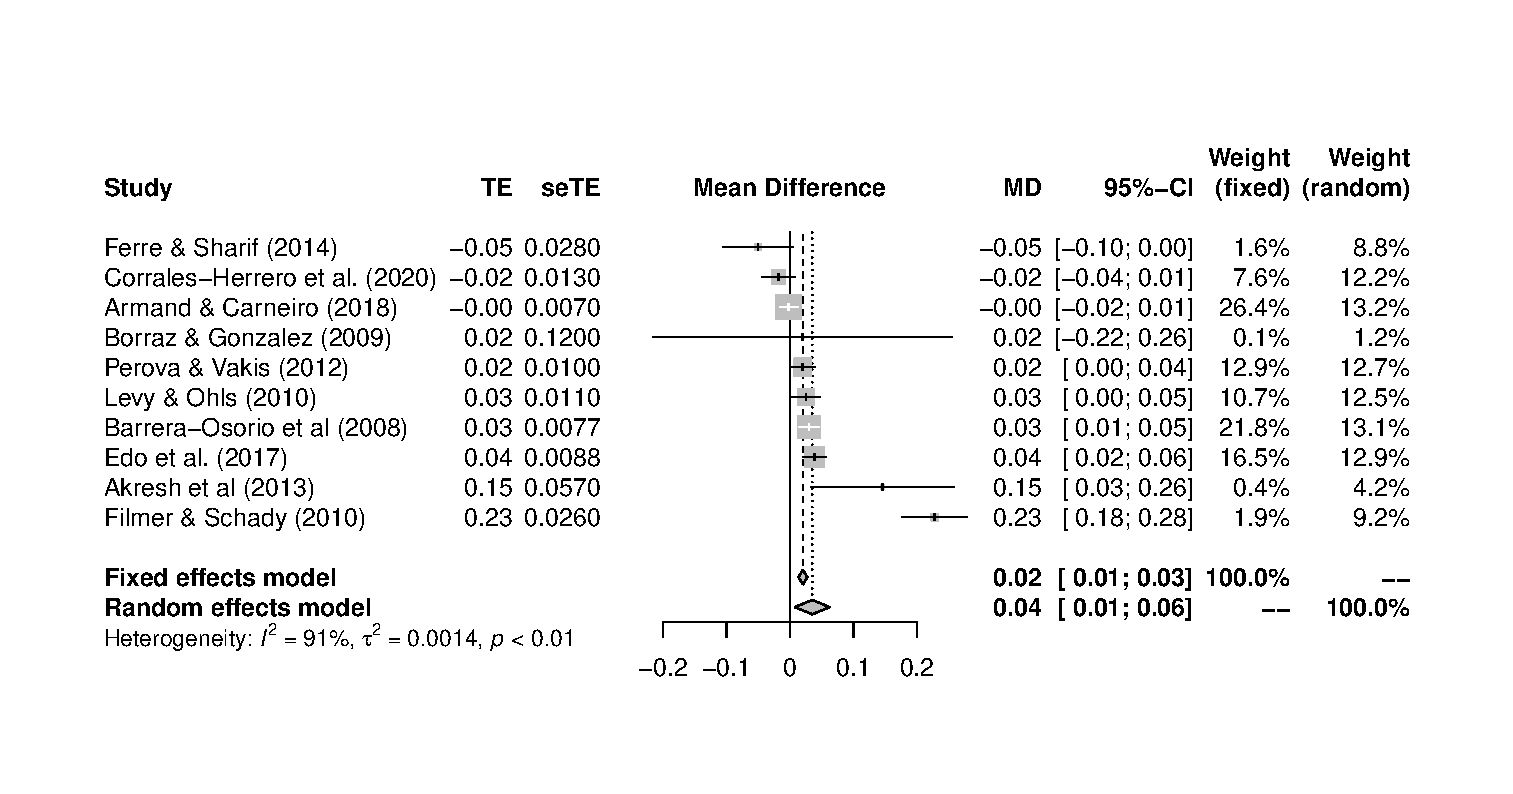
\includegraphics[width=16cm]{figures/forest_plot.pdf}
    \caption{Forest plot of the selected studies}
    \label{fig:forest}
\end{figure}


% -------------------------------------------------------------------------------------
\subsection{Evidence of Publication Bias}
In this part we explore some possible evidence of publication bias in the selected studies. The presence of publication bias could result in biased estimates of the fixed-effects and random-effects models. Therefore, it is imperative to investigate its presence and, if that is the case, to try to compensate for it.

Figure \ref{fig:funnel} shows a funnel plot of the selected studies. It appears that the selected studies are randomly distributed. However, there is a peculiar aggregation of studies sitting right on the edge of the 5\% significance level. That could be an indicator of potential publication bias. Another indicator for the presence of publication bias is the asymmetry around the estimated effect of the random-effects model. The asymmetry is an indicator of correlation between standard error and estimated effect. It appears that reported effects are symmetrically distributed with respect to the random-effects estimate. This in turn is evidence against the presence of publication bias in the selected studies.
\begin{figure}[ht]
    \centering
    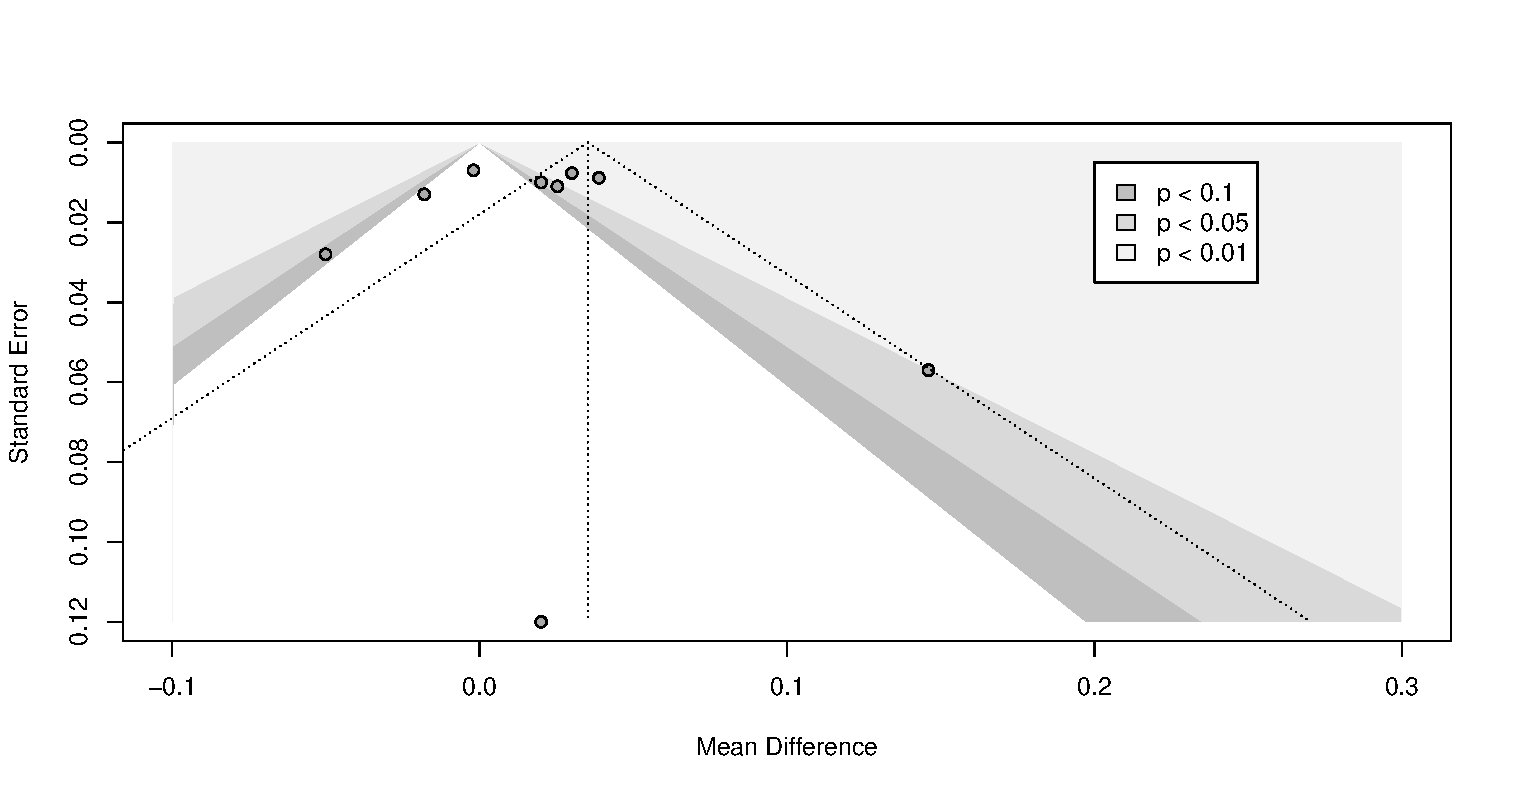
\includegraphics[width=16cm]{figures/funnel_plot.pdf}
    \caption{Funnel plot of the selected studies}
    \label{fig:funnel}
\end{figure}

We investigated the distribution of the $t$-statistics as a way to shed light on the aforementioned peculiar aggregation of studies near the edge of the 5\% significance level. Figure \ref{fig:tstat} shows the distribution and the estimated underlying normal distribution of the $t$-statistics. On the one hand, the distribution of the $t$-statistics of the selected studies peaks at 2.06, which is  extremely close to 2 and so right above the 5\% confidence threshold, indicating potential publication bias. On the other hand, the variance of the distribution is quite large, with a standard deviation of 3.16, reducing the evidence of publication bias. Overall, this findings does not allow us to neither reject nor confirm the hypothesis of publication bias.
%\wenjie{I get your point but I am just a bit confused with this underscored sentence}
%Oliver: I've just edited it. It was still the raw written text and I am fine tuning it rn
\begin{figure}[ht]
    \centering
    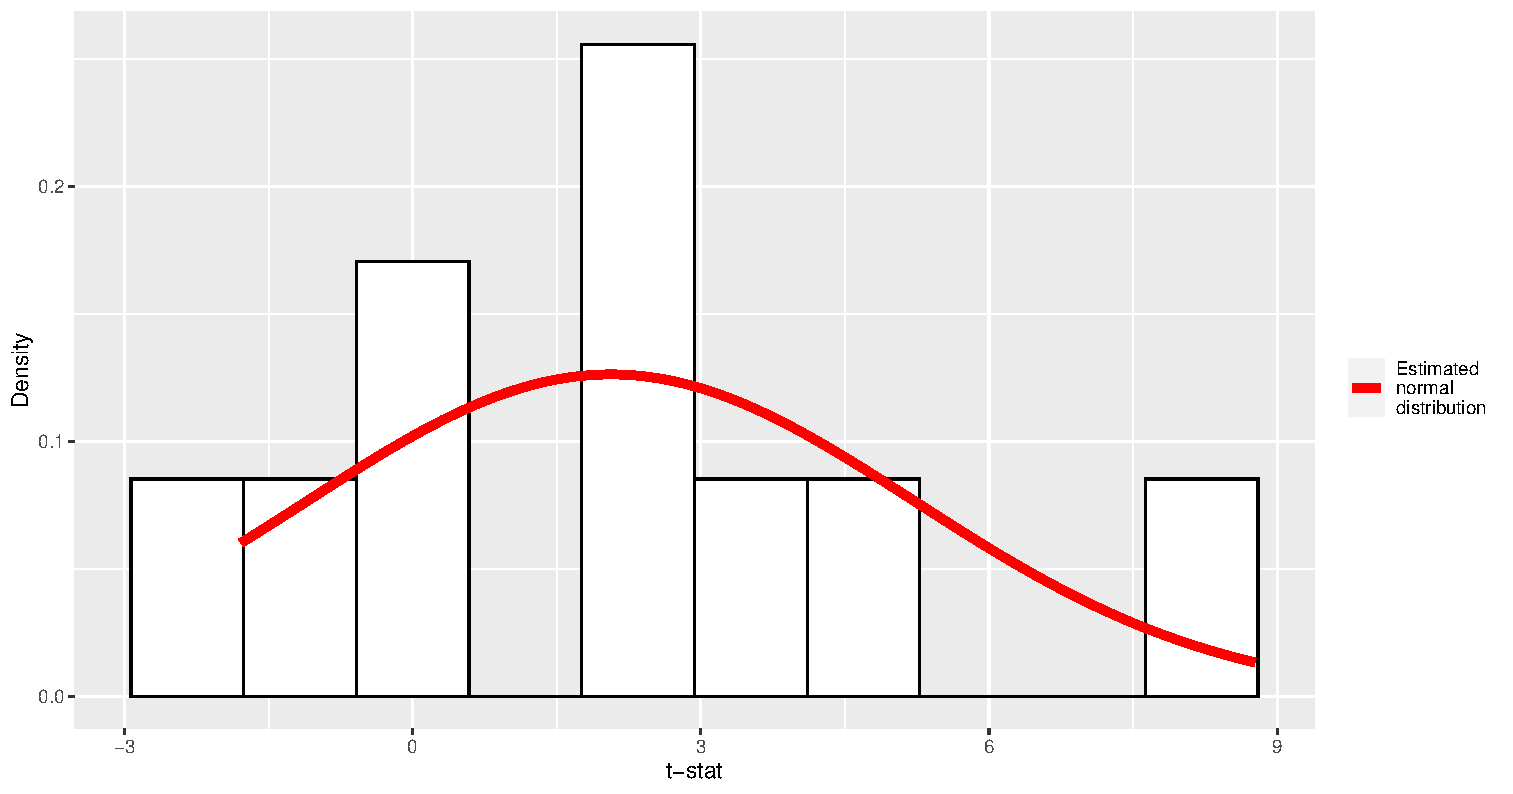
\includegraphics[width=16cm]{figures/tstat_distribution.pdf}
    \caption{$t$-statistics distribution}
    \label{fig:tstat}
\end{figure}

We tried to regress the studies' estimated effects on their standard errors to further investigate publication bias. Figure \ref{fig:effectvsse} shows a scatter plot of the estimated effect of the studies on their standard deviations with a trend line. If publication bias would not be present, we would expect the trend line to be horizontal, however we can observe a positive correlation between the reported effect and the standard error. The results of the linear regression of the effects on their standard errors are reported in table \ref{tab:effectvsse}. We find that on average the reported effects are 0.3 times the size of their standard errors and the result is not statistically different from 0. With this result we get additional evidence for publication bias not being present in our selected studies.

\begin{figure}[ht]
    \centering
    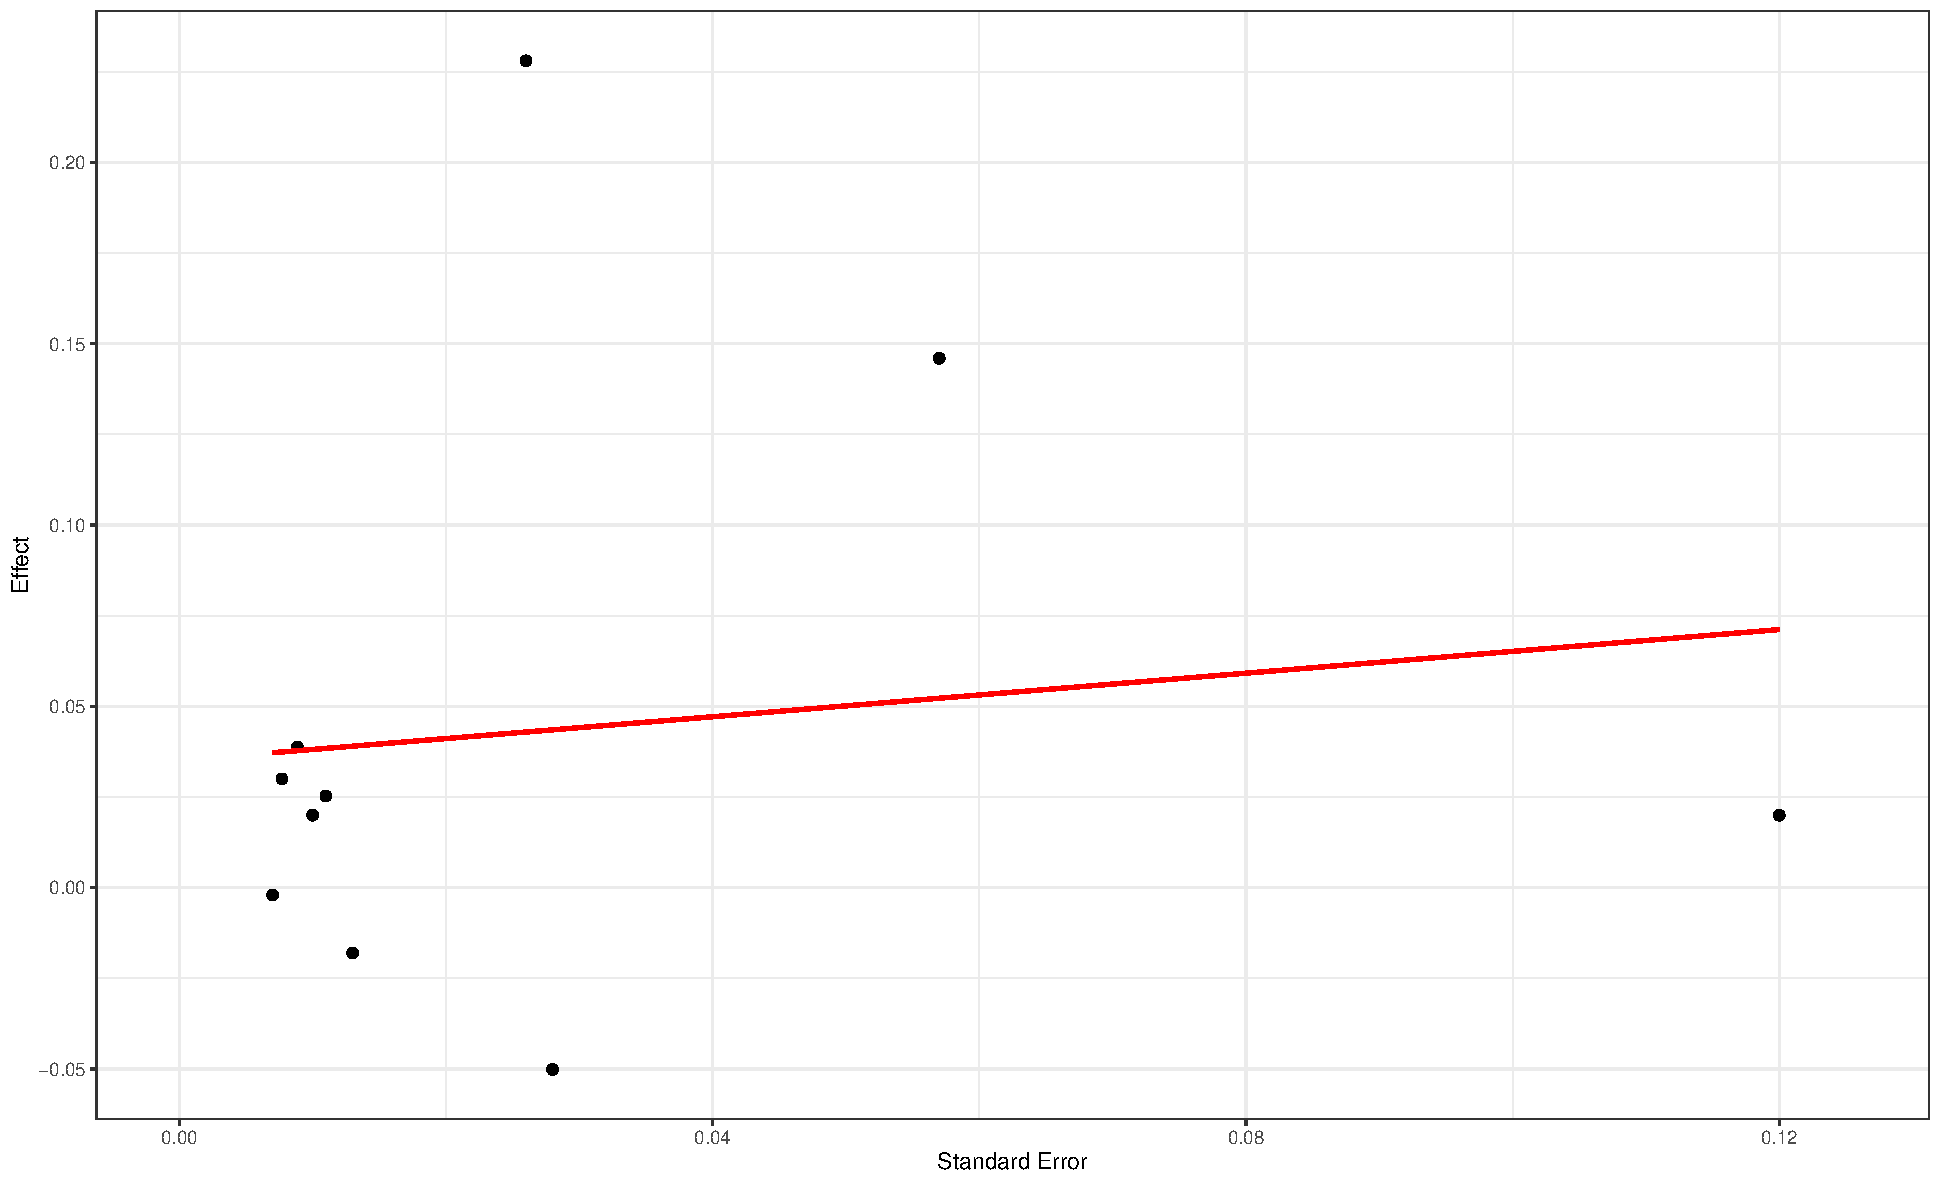
\includegraphics[width=16cm]{figures/se_effect.pdf}
    \caption{Scatter plot of the reported effects on their standard errors}
    \label{fig:effectvsse}
\end{figure}

\begin{table}[!htbp] \centering 
  \caption{Effects on SEs} 
  \label{tab:effectvsse} 
\begin{tabular}{@{\extracolsep{5pt}}lc} 
\\[-1.8ex]\hline 
\hline \\[-1.8ex] 
 & \multicolumn{1}{c}{\textit{Dependent variable:}} \\ 
\cline{2-2} 
\\[-1.8ex] & Effect \\ 
\hline \\[-1.8ex] 
 SE & 0.322 \\ 
  & (0.830) \\ 
  & \\ 
 Constant & 0.035 \\ 
  & (0.036) \\ 
  & \\ 
\hline \\[-1.8ex] 
Observations & 10 \\ 
\hline 
\hline \\[-1.8ex] 
\textit{Note:}  & \multicolumn{1}{r}{$^{*}$p$<$0.1; $^{**}$p$<$0.05; $^{***}$p$<$0.01} \\ 
\end{tabular} 
\end{table} 

Overall, we did not find any strong evidence of publication bias being present in our selected studies, just some hints for it. On the other hand, we have important evidence against the publication bias hypothesis. Therefore, we feel confident that we can reject the publication bias hypothesis.


% -------------------------------------------------------------------------------------

\subsection{Correcting for Publication Bias and Heterogeneity}
We ran a series of meta-regressions to account for between-study heterogeneity. We also tried to add controls for publication bias in some of them, even though we refuted the hypothesis in the last subsection. We just want to be sure that we are not making a mistake. We assumed a linear association between the reported effects and their standard errors when attempting to correct for publication bias. First, we developed three linear models to attempt to correct for between-study heterogeneity, then we added controls for publication bias. In all meta-regressions, the constant term $\beta_0$ represents the estimated underlying real effect of the treatment.

Since a large amount of the selected studies was conducted in South America, we wanted to add a dummy variable for the continent. We would have liked to add dummy variables for the other continents as well, but the small sample size does not allow it. We estimated the following meta-regression:
\begin{equation}
    ReportedEffect_i = \beta_0 + \beta_1 SouthAmerica_i + \varepsilon_i,
\end{equation}
where $SouthAmerica_i$ is a dummy variable that takes value 1 if the study was conducted in South America and is 0 otherwise. The results are reported in column (1) of table \ref{tab:metaregs}. The estimated real effect and the coefficient on the control variable are not statistically significant.

As two of our hypothesis about the causes of heterogeneity were that there might have been changes over time and differences in CCT programs, we ran another meta-regression dividing the studies in two categories: studies from 2012 or before, and studies that have been published after 2012. We opted for such partition as it allows to have some studies in both categories (before and after) and it is in line with the start of the European Debt Crisis, which could have had an impact on the founding of CCT programs. We estimated the following regression:
\begin{equation}
    ReportedEffect_i = \beta_0 + \beta_1 after2012_i + \varepsilon_i,
\end{equation}
where $after2012_i$ is a dummy variable for studies that have been published after 2012. The regression results are reported in column (2) of table \ref{tab:metaregs}. We did not find any significance neither of the estimated real effect nor of the coefficient on the control variable.

We also tried to run a meta-regression that includes both control variables,
\begin{equation}
    ReportedEffect_i = \beta_0 + \beta_1 SouthAmerica_i + \beta_2 after2012_i + \varepsilon_i.
\end{equation}
The results are reported in column (3) of table \ref{tab:metaregs}, but no statistical significance is found on any coefficient.

In the remaining part of this subsection we report meta-regression models for which we added controls for publication bias. In the previous subsection we did not find strong evidence of the presence of publication bias and were inclined to discard the hypothesis, but we still want to control for it just to be sure. The first meta-regression we ran in this setting is
\begin{equation}
    ReportedEffect_i = \beta_0 + \beta_1 SE_i + \varepsilon_i,
\end{equation}
in which $SE_i$ is the standard error of the reported effect. This model happens to be the same model as the one reported in table \ref{tab:effectvsse}. The results are in column (4) of table \ref{tab:metaregs} and show no statistical significance of any coefficient.

Then we added the control variable for South American countries:
\begin{equation}
    ReportedEffect_i = \beta_0 + \beta_1 SouthAmerica_i + \beta_2 SE_i + \varepsilon_i.
\end{equation}
The results are reported in column (5) of table \ref{tab:metaregs} and once more they show no significance.

After that, we tried with the control variable for sutdies after 2012:
\begin{equation}
    ReportedEffect_i = \beta_0 + \beta_1 after2012_i + \beta_2 SE_i + \varepsilon_i.
\end{equation}
The results are reported in column (6) of table \ref{tab:metaregs} and are not statistically significant.

Finally, we included all controls in a single meta-regression:
\begin{equation}
    ReportedEffect_i = \beta_0 + \beta_1 SotuhAmerica_i + \beta_2 after2012_i + \beta_3 SE_i + \varepsilon_i.
\end{equation}
Column (7) of table \ref{tab:effectvsse} reports the result. The pattern repeats and all the results are not statistically significant.

Overall, we were not able to control for heterogeneity. This might be due the small sample size of studies or the unavailability of other data to control for. On a final note, we also did not find any evidence of publication bias in this part, therefore we are inclined to support our findings in figure \ref{fig:forest} of the random-effects model.


\begin{table}[!htbp] \centering 
  \caption{Results of the meta-regressions} 
  \label{tab:metaregs} 
\begin{tabular}{@{\extracolsep{5pt}}lccccccc} 
\\[-1.8ex]\hline 
\hline \\[-1.8ex] 
 & \multicolumn{7}{c}{\textit{Dependent variable:}} \\ 
\cline{2-8} 
\\[-1.8ex] & \multicolumn{7}{c}{Effect} \\ 
\\[-1.8ex] & (1) & (2) & (3) & (4) & (5) & (6) & (7)\\ 
\hline \\[-1.8ex] 
 SouthAmerica & 0.047 &  & 0.035 &  & 0.045 &  & 0.033 \\ 
  & (0.053) &  & (0.070) &  & (0.057) &  & (0.075) \\ 
  & & & & & & & \\ 
 after2012 &  & $-$0.042 & $-$0.021 &  &  & $-$0.039 & $-$0.020 \\ 
  &  & (0.053) & (0.070) &  &  & (0.057) & (0.075) \\ 
  & & & & & & & \\ 
 SE &  &  &  & 0.322 & 0.211 & 0.218 & 0.187 \\ 
  &  &  &  & (0.830) & (0.862) & (0.873) & (0.931) \\ 
  & & & & & & & \\ 
 RealEffect & 0.020 & 0.065 & 0.037 & 0.035 & 0.015 & 0.057 & 0.031 \\ 
  & (0.037) & (0.038) & (0.068) & (0.036) & (0.044) & (0.050) & (0.079) \\ 
  & & & & & & & \\ 
\hline \\[-1.8ex] 
Observations & 10 & 10 & 10 & 10 & 10 & 10 & 10 \\ 
R$^{2}$ & 0.091 & 0.072 & 0.103 & 0.018 & 0.099 & 0.080 & 0.109 \\ 
Adjusted R$^{2}$ & $-$0.022 & $-$0.044 & $-$0.153 & $-$0.104 & $-$0.158 & $-$0.183 & $-$0.337 \\ 
\hline 
\hline \\[-1.8ex] 
\textit{Note:}  & \multicolumn{7}{r}{$^{*}$p$<$0.1; $^{**}$p$<$0.05; $^{***}$p$<$0.01} \\ 
\end{tabular}
\end{table}

% -------------------------------------------------------------------------------------


% -------------------------------------------------------------------------------------
\section{Conclusion} \label{sec:conclusion}
Our meta-analytical research found a positive impact of CCT programs on school attendance. The random-effects model points at an increase of 4 percentage points following the introduction of CCTs. We tried to control for continental and temporal effects, but we found no statistical significance of the control variables. Therefore, the high level of heterogeneity remains unaddressed. We also investigated publication bias and found no evidence of it being present in our selected studies, reinforcing the robustness of our results.

\clearpage

\nocite{*}
\bibliographystyle{apalike}
\bibliography{references}


\newpage

\appendix
\section*{Summaries of the Selected Studies}

\paragraph{Akresh et al (2013)}

Authors estimate the impact of cash transfers on education by conducting a randomized experiment in rural Burkina Faso. The two-year pilot program randomly distributed cash transfers that were either conditional or unconditional. Families under the conditional schemes were required to have their children ages 7–15 enrolled in school and attending classes regularly. There were no such requirements under the unconditional schemes. The results show that unconditional and conditional cash transfer programs have a similar impact increasing the enrollment of children who are traditionally favored by parents for school participation, including boys, older children, and higher-ability children. The conditional transfers, however, are significantly more effective than the unconditional transfers in improving the enrollment of ``marginal children'' who are initially less likely to go to school, such as girls, younger children, and lower-ability children. Hence, it is concluded that conditionality plays a critical role in benefiting children who are less likely to receive investments from their parents.

% Authors conduct a natural experiment in rural Burkina Faso to estimate the impact of cash transfers on education. The two-year pilot program randomly distributed cash transfers that were either conditional or unconditional. Families under the conditional schemes were required to have their children ages 7–15 enrolled in school and attending classes regularly. There were no such requirements under the unconditional programs. The results indicate that unconditional and conditional cash transfer programs have a similar impact increasing the enrollment of children who are traditionally favored by parents for school participation, including boys, older children, and higher ability children. However, the conditional transfers are significantly more effective than the unconditional transfers in improving the enrollment of ``marginal children'' who are initially less likely to go to school, such as girls, younger children, and lower ability children. Thus, conditionality plays a critical role in benefiting children who are less likely to receive investments from their parents.

\paragraph{Armand \& Carneiro (2018)}

This paper examines the short- and medium-run the conditional cash transfer and its modalities on school enrollment. The results show that CCT has strong impacts on school enrolment among children of secondary school age, but not on school attendance. There are no substantial differences in household or child outcomes between receiving the payments in equal instalments or having a graduation bonus.

\paragraph{Barrera-Osorio et al (2008)}

This paper evaluates multiple variants of a commonly used intervention (conditional cash transfer) to boost education in developing countries. Authors conduct a randomized experiment at a student level, which allows for intra-family and peer-network variation. They test three treatments: a basic CCT treatment based on school attendance, a savings treatment that postpones a bulk of the cash transfer due to good attendance to just before children have to reenroll, and a tertiary treatment where some of the transfers are conditional on students' graduation and tertiary enrollment rather than attendance. On average, the combined incentives increase attendance, pass rates, enrollment, graduation rates, and matriculation to tertiary institutions. Changing the timing of the payments does not change attendance rates relative to the basic treatment but does significantly increase enrollment rates at both the secondary and tertiary levels. Incentives for graduation and matriculation are particularly effective, increasing attendance and enrollment at secondary and tertiary levels more than the basic treatment. They find some evidence that the subsidies can cause a reallocation of responsibilities within the household. Siblings (particularly sisters) of treated students work more and attend school less than students in families that received no treatment. They also find that indirect peer influences are relatively strong in attendance decisions with the average magnitude similar to that of the direct effect.

\paragraph{Borraz \& Gonzalez (2009)}

In this paper, authors analyze the impact of conditional cash payments on school enrollment, child labor and labor supply implemented between 2005 and 2007 to the poorest Uruguayan households. Targeting income discontinuities are not observed around the thresholds to participate in the program, which invalidates the use of regression discontinuity designs for evaluating causal effects of the intervention. They instead apply the propensity score matching estimator to account for the endogeneity of program participation. They find that the program has no impact on school attendance but reduces female child labor in Montevideo. In addition negative effects are detected on the labor market in the rest of the urban areas.

\paragraph{Corrales-Herrero et al. (2020)}

This paper is to evaluate the impact of the Red de Oportunidades program on the school attendance of children from households that participate in the program. Authors apply propensity score matching, a quasi-experimental technique that allows them to find an appropriate control group to compare with the treatment group. They find that the program does not always manage to bring into line school attendance of children from families involved in the program  with that of children from families who are not. Nevertheless, differences are still evident in terms of age, gender and geographical area. They conclude that CCT programs should be designed carefully, taking into account a great variety of factors such as geographical characteristics, educational resources and infrastructure, not only to replicate programs that have proved to be effective in other countries. In this sense, it seems that the impact of cash transfers on primary school attendance can be wholly attributed to the program, implying that it is better to allocate more resources to groups in terms of age and gender where education is still not universal.

\paragraph{Edo et al. (2017)}

In this paper, authors claim that the Asignación Universal por Hijo (Universal Child Allowance, AUH) — a massive conditional cash transfer program implemented in 2009 in Argentina — may be mostly responsible for the improvement in school attendance rates for children aged 15 through 17. By using a difference-in-differences strategy, they estimate that the program accounts for a 3.9 percentage point increase in the probability of attending secondary school among eligible children aged 15 through 17. The impact seems to be led by boys and is more relevant for children living in larger families where the head of household has a lower educational level.

\paragraph{Ferre \& Sharif (2014)}

This paper uses panel data from a pilot project and evaluates the impact of conditional cash transfers on consumption, education, and nutrition outcomes among poor rural families in Bangladesh. Given implementation challenges, the intervention was not able to improve school attendance. However the analysis shows that the pilot had a significant impact on the incidence of wasting among children who were 10–22 months old when the program started, reducing the share of children with weight-for-height below two standard deviations from the World Health Organization benchmark by 40 percent. The pilot was also able to improve nutrition knowledge: there was a significant increase in the proportion of beneficiary mothers who knew about the importance of exclusively breastfeeding infants until the age of six months. The results also suggest a significant positive impact on food consumption, especially consumption of food with high protein content.

\paragraph{Filmer \& Schady (2010)}

In this paper, authors analyze the impact of a program in Cambodia that made payments of varying magnitude to otherwise comparable households. The identification is based on a sharp regression discontinuity design. They find that a modest cash transfer, equivalent to approximately 2\% of the consumption of the median recipient household, had a substantial impact on school attendance, approximately 25 percentage points. A somewhat larger transfer did not raise attendance rates above this level.

\paragraph{Levy \& Ohls (2010)}

This paper summarizes the findings of an evaluation of the Program of Advancement through Health and Education (PATH), a CCT program implemented by the Government of Jamaica. The authors find that PATH was generally implemented as intended; exhibited better targeting to the poor than other similar social assistance programs in Jamaica; and had positive and statistically significant impacts on school attendance and number of preventive healthcare visits for children. They find no evidence, however, that PATH was able to affect longer-term outcomes such as marks, grade progression, or healthcare status.

\paragraph{Perova \& Vakis (2012)}

This study presents results from a quantitative impact evaluation of the Conditional Cash Transfer (CCT) program, Juntos, in Peru. Using instrumental variable techniques, it estimates the overall impact of Juntos five years after its initial rollout and explores the differential impacts among beneficiaries according to the length of time they spent in the program. In so doing, the analysis explores whether it takes time for the program to make significant and sizable impacts; and whether some impacts change in magnitude the longer the beneficiaries spend in the program. The results seem to confirm both hypotheses: almost all indicators of interest are significantly higher among beneficiaries with longer treatment spells. However, in many cases these improvements are too small to be picked up in the analysis of overall effects, when beneficiaries are compared to non-beneficiaries. These findings suggest that while the program has a non negligible impact on welfare, there is room for improvement.


% -------------------------------------------------------------------------------------

\end{document}
